% ------------------------------------------------------------------------
% ------------------------------------------------------------------------
% abnTeX2: Modelo de Artigo Acadêmico em conformidade com
% ABNT NBR 6022:2003: Informação e documentação - Artigo em publicação 
% periódica científica impressa - Apresentação
% ------------------------------------------------------------------------
% ------------------------------------------------------------------------

\documentclass[
	% -- opções da classe memoir --
	article,			% indica que é um artigo acadêmico
	12pt,				% tamanho da fonte
	oneside,			% para impressão apenas no verso. Oposto a twoside
	a4paper,			% tamanho do papel. 
	% -- opções da classe abntex2 --
	%chapter=TITLE,		% títulos de capítulos convertidos em letras maiúsculas
	%section=TITLE,		% títulos de seções convertidos em letras maiúsculas
	%subsection=TITLE,	% títulos de subseções convertidos em letras maiúsculas
	%subsubsection=TITLE % títulos de subsubseções convertidos em letras maiúsculas
	% -- opções do pacote babel --
	english,			% idioma adicional para hifenização
	brazil,				% o último idioma é o principal do documento
	sumario=tradicional
	]{abntex2}


% ---
% PACOTES
% ---

% ---
% Pacotes fundamentais 
% ---
\usepackage{lmodern}			% Usa a fonte Latin Modern
\usepackage[T1]{fontenc}		% Selecao de codigos de fonte.
\usepackage[utf8]{inputenc}		% Codificacao do documento (conversão automática dos acentos)
\usepackage{indentfirst}		% Indenta o primeiro parágrafo de cada seção.
\usepackage{nomencl} 			% Lista de simbolos
\usepackage{color}				% Controle das cores
\usepackage{graphicx}			% Inclusão de gráficos
\usepackage{microtype} 			% para melhorias de justificação
% ---
		
% ---
% Pacotes adicionais, usados apenas no âmbito do Modelo Canônico do abnteX2
% ---
\usepackage{lipsum}				% para geração de dummy text
\usepackage{subcaption}


% ---
		
% ---
% Pacotes de citações
% ---
\usepackage[brazilian,hyperpageref]{backref}	 % Paginas com as citações na bibl
\usepackage[alf]{abntex2cite}	% Citações padrão ABNT
% ---

% ---
% Configurações do pacote backref
% Usado sem a opção hyperpageref de backref
\renewcommand{\backrefpagesname}{Citado na(s) página(s):~}
% Texto padrão antes do número das páginas
\renewcommand{\backref}{}
% Define os textos da citação
\renewcommand*{\backrefalt}[4]{
	\ifcase #1 %
		Nenhuma citação no texto.%
	\or
		Citado na página #2.%
	\else
		Citado #1 vezes nas páginas #2.%
	\fi}%
% ---

% ---
% Informações de dados para CAPA e FOLHA DE ROSTO
% ---
\titulo{Breve Estudo da Fotografia Astronômica}
\autor{Esron Dtamar da Silva}
\local{Brasil}
\data{\today}
% ---

% ---
% Configurações de aparência do PDF final

% alterando o aspecto da cor azul
\definecolor{blue}{RGB}{41,5,195}

% informações do PDF
\makeatletter
\hypersetup{
     	%pagebackref=true,
		pdftitle={\@title}, 
		pdfauthor={\@author},
    	pdfsubject={},
	    pdfcreator={LaTeX with abnTeX2},
		pdfkeywords={abnt}{latex}{abntex}{abntex2}{atigo científico}, 
		colorlinks=true,       		% false: boxed links; true: colored links
    	linkcolor=blue,          	% color of internal links
    	citecolor=blue,        		% color of links to bibliography
    	filecolor=magenta,      		% color of file links
		urlcolor=blue,
		bookmarksdepth=4
}
\makeatother
% --- 

% ---
% compila o indice
% ---
\makeindex
% ---

% ---
% Altera as margens padrões
% ---
\setlrmarginsandblock{3cm}{3cm}{*}
\setulmarginsandblock{3cm}{3cm}{*}
\checkandfixthelayout
% ---

% --- 
% Espaçamentos entre linhas e parágrafos 
% --- 

% O tamanho do parágrafo é dado por:
\setlength{\parindent}{1.3cm}

% Controle do espaçamento entre um parágrafo e outro:
\setlength{\parskip}{0.2cm}  % tente também \onelineskip

% Espaçamento simples
\SingleSpacing

% ----
% Início do documento
% ----
\begin{document}

% Retira espaço extra obsoleto entre as frases.
\frenchspacing 

% ----------------------------------------------------------
% ELEMENTOS PRÉ-TEXTUAIS
% ----------------------------------------------------------

%---
%
% Se desejar escrever o artigo em duas colunas, descomente a linha abaixo
% e a linha com o texto ``FIM DE ARTIGO EM DUAS COLUNAS''.
% \twocolumn[    		% INICIO DE ARTIGO EM DUAS COLUNAS
%
%---
% página de titulo
\maketitle

% resumo em português
\begin{resumoumacoluna}
 Conforme a hue hue BR 6022:2003, o resumo é elemento obrigatório, constituído de
 uma sequência de frases concisas e objetivas e não de uma simples enumeração
 de tópicos, não ultrapassando 250 palavras, seguido, logo abaixo, das palavras
 representativas do conteúdo do trabalho, isto é, palavras-chave e/ou
 descritores, conforme a NBR 6028. (\ldots) As palavras-chave devem figurar logo
 abaixo do resumo, antecedidas da expressão Palavras-chave:, separadas entre si por
 ponto e finalizadas também por ponto.
 
 \vspace{\onelineskip}
 
 \noindent
 \textbf{Palavras-chaves}: latex. abntex. editoração de texto.
\end{resumoumacoluna}

% ----------------------------------------------------------
% ELEMENTOS TEXTUAIS
% ----------------------------------------------------------
\textual

% ----------------------------------------------------------
% Introdução
% ----------------------------------------------------------
\section*{O pensamento em preto-e-branco}
\addcontentsline{toc}{section}{O pensamento em preto-e-branco}


A definição mais básica para fotografia em preto e branco é a ausência de qualquer cor na foto. A fotografia em preto e branco é uma fotografia monocromática, porém, a reciproca não é verdadeira. Por exemplo, há fotografias monocromáticas que possuem tons de amarelo e vermelho (sépia), outras em tons de azul. Porém, um fotografia só se torna uma foto em preto-e-branco se os tons forem cinzas. De acordo com \citeonline{SITEGURUSHOTS} você deve se treinar a ver em tons se deseja se tornar profissional nesse tipo de fotografia. \citeonline{SITEMASTERING} destaca que ver sem cores é focar sua atenção nas formas e  sombras, e pensar em como elas trabalham na composição. Mesmo quando há pouca luz e formas pouco definidas, esses elementos permanecem como motores principais do sentido da fotografia. Além disso, o autor também destaca que nos casos de pouca luminosidade, os fatores citados anteriormente se tornam mais integrados, seja na relação forma para o \textit{frame}, forma para o ambiente ou forma para forma, pois no preto-e-branco esses relacionamentos se tornam mais evidentes que na cor.
\citeonline{SITE7TIPS} diz que se você deseja imagens com um contraste muito alto e uma gradação de tons muito elevados também, deve-se utilizar luz dura. Por outro lado, se é desejável obter tons suaves e imagens sutis, a escolha deve ser de uma luz difusa.

\citeonline{SITEGURUSHOTS} considera a existência de 5 pilares para a fotografia em preto-e-branco, são eles: contraste, tons, texturas, formas e sombras. Entretanto, para o retrato em preto e branco, que é a proposta desse artigo, serão considerados os seguintes elementos: iluminação, expressão, composição e pós-processamento.

% ----------------------------------------------------------
% Seção de explicações
% ----------------------------------------------------------
\section{Os elementos do retrato preto-e-branco}

\subsection{A iluminação básica para o retrato}

Segundo \citeonline{SITE6LUZ}, existem 6 (seis) padrões de iluminação clássicos a captura de um retrato. Padrão de iluminação é, de uma maneira resumida, a forma como a luz interage com as características faciais do modelo, criando áreas de luz e sombra. 
O que diferencia os padrões de iluminação é a forma da sombra criada no rosto do modelo. Os padrões de iluminação são a luz curta, luz ampla, luz borboleta, luz dividida, luz de \textit{loop} e a luz de Rembrandt. Abaixo são descritas brevemente as formas de iluminação, ao passo que são exemplificadas pela figura \ref{img:classic}.

\begin{itemize}
	\item A luz curta é utilizada para gerar uma sombra no lado do rosto do modelo mais próximo a câmera (figura \ref{img:short}).
	\item Ao contrário da luz curta, a luz ampla forma sombra no lado mais distante do rosto do modelo (figura \ref{img:broad}).
	\item A luz borboleta é caracterizada pela forma de borboleta gerada sob o nariz do modelo (figura \ref{img:butter}).
	\item A luz dividida possui esse nome porque divide o rosto do modelo em dois lados iguais, um iluminado e outro sombreado (figura \ref{img:split}).
	\item Na luz de loop são geradas pequenas sombras no nariz e bochechas do modelo (figura \ref{img:loop}).
	\item A luz de Rembrandt é definida pelo triângulo de luz formado na bochecha do modelo (figura \ref{img:rembrandt}). 
\end{itemize}

Todos esses padrões de iluminação são obtidos variando a posição da fonte luminosa em relação ao modelo, seja horizontalmente ou verticalmente. Porém esse assunto não será abordado aqui, pois tal abordagem profunda foge do escopo desse artigo.

\begin{figure}[!htb]
\centering
    \caption{\label{img:classic} Iluminações clássicas para o retrato}
    \subcaptionbox{\label{img:short} Luz curta}{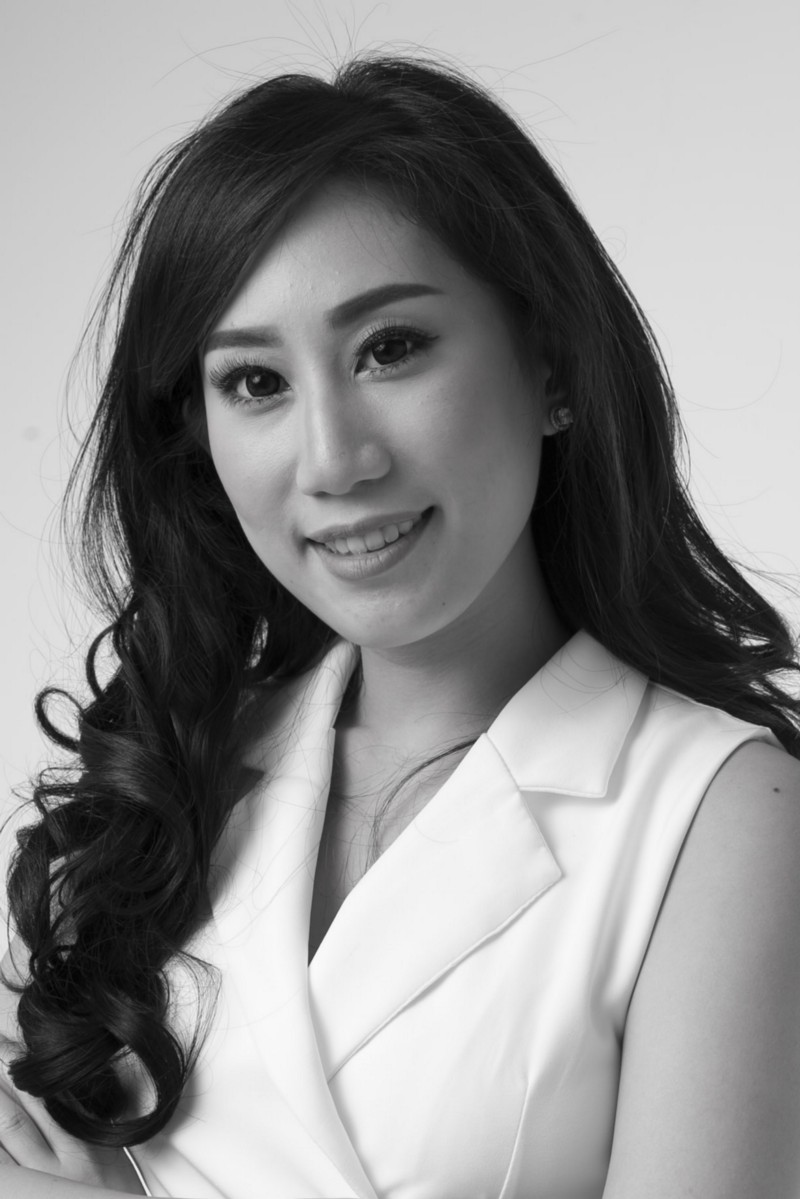
\includegraphics[scale=.15]{img/short}}\qquad
    \subcaptionbox{\label{img:broad} Luz ampla}{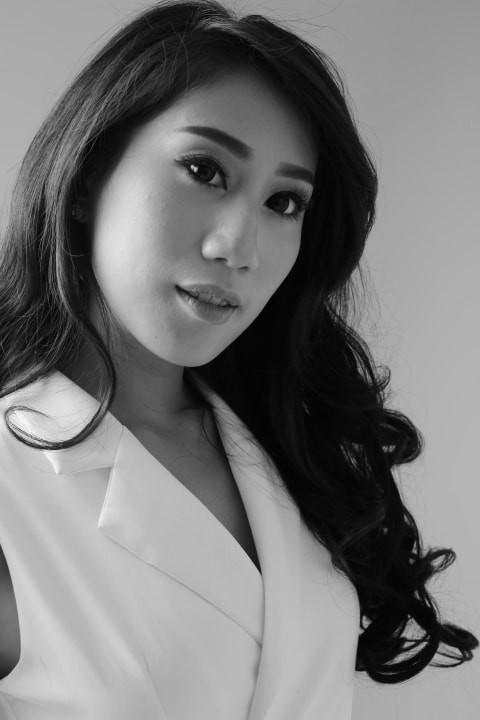
\includegraphics[scale=.25]{img/broad}}\qquad
    \subcaptionbox{\label{img:butter} Luz borboleta}{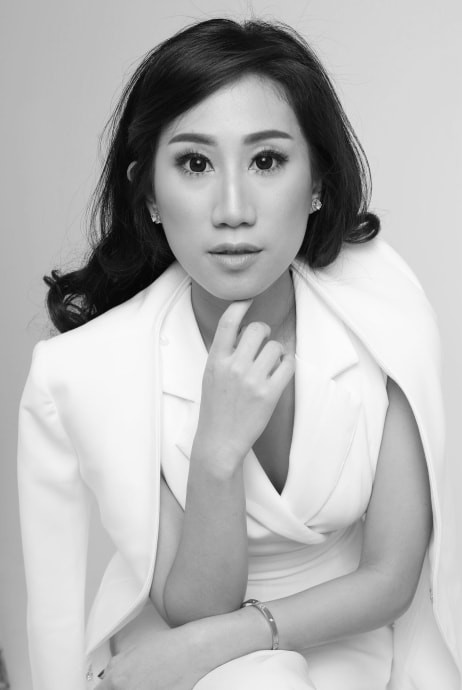
\includegraphics[scale=.26]{img/butter}}\\
    \vspace{1.5em}
    \subcaptionbox{\label{img:split} Luz dividida}{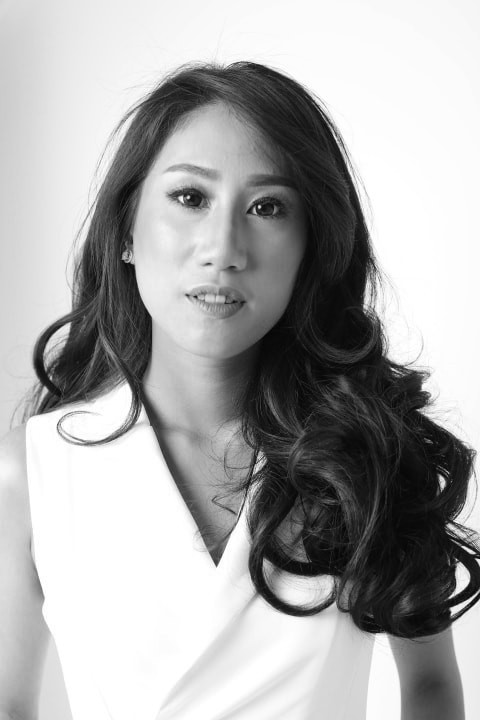
\includegraphics[scale=.25]{img/split}}\qquad
    \subcaptionbox{\label{img:loop} Luz de \textit{loop}}{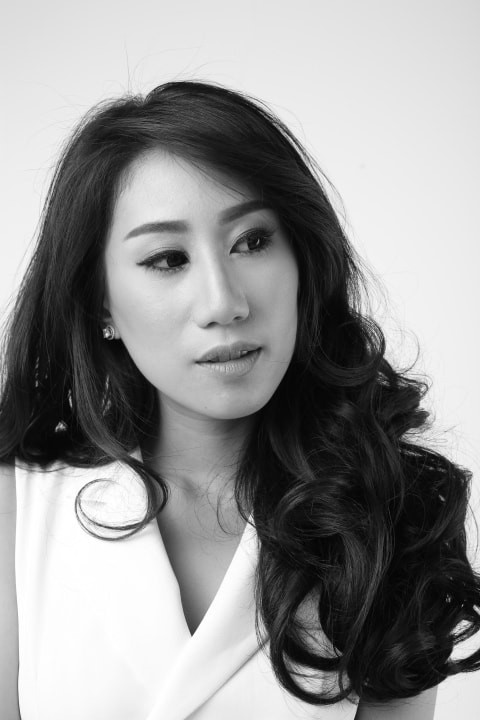
\includegraphics[scale=.25]{img/loop}}\qquad
    \subcaptionbox{\label{img:rembrandt} Luz de Rembrandt}{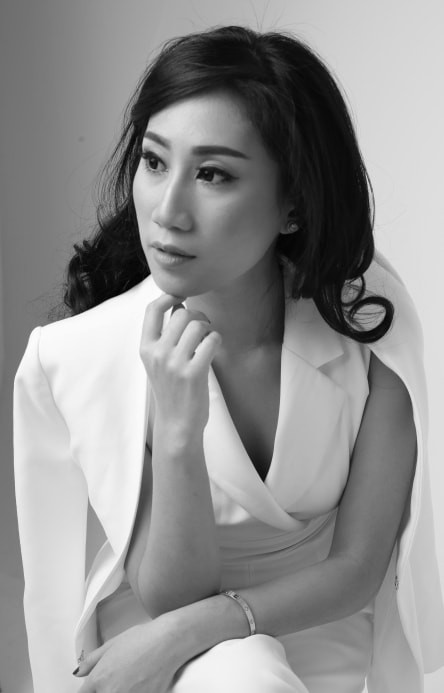
\includegraphics[scale=.26]{img/rembrandt}}\\
    \vspace{2.5em}
    \legend{\textbf{Fonte:} \cite{SITE6LUZ}}
\label{fig:dag}
\end{figure}

\newpage

\subsection{A expressão}

Segundo \citeonline{SITE7TIPS}, a omissão da cor provoca a divisão da imagem em preto-e-branco em formas e formas-gráficas. Devido a isso, a expressão do assunto, por menor que seja, se torna mais proeminente, como por exemplo uma sobrancelha levantada, rugas e até mesmo uma contração no canto da boca. 

\begin{citacao}
	"...eyes are a window on the soul" \citeonline{SITEGURUSHOTS}
\end{citacao}

Entretanto, o autor destaca fortemente que a parte mais importante da expressão são os olhos. Os olhos são utilizados comumente como ponto focal e sua fotografia deve ser construída em torno deles. As formas dos olhos são facilmente reconhecidas e capturam imediatamente a atenção do observador. Desta forma, é muito importante que eles estejam focados e bem iluminados.

De acordo com \citeonline{SITE5TIPS}, é interessante que se tenha um contato maior com o modelo, no sentido de explorar uma conversa e prestar atenção nas expressões do modelo quando determinados assuntos são colocados em pauta, para então tentar capturar aquele momento íntimo e revelar o verdadeiro caráter do modelo.

\subsection{A composição}

A mensagem deste tópico é, mantenha a composição o mais simples possível. A própria fotografia em preto-e-branco é uma simplificação na composição, pois remove a cor da cena. É importante manter o fundo o mais organizado possível, mesmo que isso signifique se aproximar do modelo ou usar uma grande abertura para desfocar o fundo, consequentemente removendo distrações e chamando a atenção para o modelo \cite{SITE5TIPS}.

Como dito anteriormente, a expressão, o olhar e a iluminação sobre o modelo devem estar em ressonância para se obter uma boa composição através das formas geradas, sombras, valores tonais e demais fatores, porém sempre tendo em mente que o objeto da foto é o modelo.

\subsection{Pós-processamento}

Quando se trata de edição, é necessário saber explorar as várias opções que o \textit{software} adotado fornece. Converter um retrato para preto-e-branco, pode não resultar em uma imagem atraente até que seja realizados os ajustes de tons, curvas e claridade necessários. Tais ajuste permitem o aprofundamento das sombras e a claridade dos realces da foto.Uma outra possibilidade é adicionar um pouco de ruído, simulando a captura através de uma câmera analógica antiga \cite{SITEEXPERT}.

Em relação aos ajustes, há de se ter um cuidado quando se ajusta a claridade de uma imagem, por um lado, as texturas se tornam mais evidentes, o que é um ponto positivo para a fotografia em preto-e-branco. Por outro lado, aumentar demais a claridade pode tornar os tons de pele texturizado demais, isso é um problema especialmente para modelos femininas, onde se espera uma pele mais suave \cite{SITE5TIPS}.

No pós-processamento não há uma "receita de bolo", muitas das edições dependem unicamente da criatividade do autor. É claro que existem alguns passos básicos como citados anteriormente, tais como correção de tons, contraste, exposição e dentre outros, mas o que torna a imagem única é encontrar o processo que atende o gosto pessoal de cada fotógrafo. 

% ---
% Finaliza a parte no bookmark do PDF, para que se inicie o bookmark na raiz
% ---
\bookmarksetup{startatroot}% 
% ---

% ---
% Conclusão
% ---
\section*{Considerações finais}
\addcontentsline{toc}{section}{Considerações finais}

\lipsum[1]

\begin{citacao}
\lipsum[2]
\end{citacao}

\lipsum[3]
\newpage
% ----------------------------------------------------------
% ELEMENTOS PÓS-TEXTUAIS
% ----------------------------------------------------------
\postextual

% ----------------------------------------------------------
% Referências bibliográficas
% ----------------------------------------------------------
\bibliography{abntex2-modelo-references}


\end{document}
